\section{Diagramas de flujo de datos}

  \paragraph{}Los diagramas de flujo de datos son una representación gráfica en
  forma de red que refleja el flujo de la información y las transformaciones que
  se aplican sobre ella al moverse desde la entrada hasta la salida de un
  sistema software. Un DFD representa qué funciones o qué transformaciones deben
  realizarse sobre los datos, pero no cuándo se realizan o en qué orden.

  \paragraph{}Los diagramas de flujo de datos ayudan a modelar las funciones que
  debe realizar el sistema, permitiendo una descomposición funcional del sistema
  en distintos niveles de detalle.

  \paragraph{}El refinamiento de estos diagramas se hace mediante niveles,
  comenzando por el nivel 0 o diagrama de contexto del sistema y finalizando en
  un nivel que ya no pueda descomponerse más debido a su sencillez.

  \paragraph{}Existen diferentes metodologías para la representación de los
  diagramas de flujo de datos, aquí se usará la metodología de Yourdon-DeMarco
  por ser una de las más extendidas.

  \paragraph{}La notación básica de esta metodología hace uso de los siguientes
  componentes: el proceso (que se clasifica en simple o compuesto), el flujo, el
  almacén y la entidad externa.

  \begin{description}
   \item[Proceso simple] El proceso simple se representa gráficamente mediante
        un círculo blanco y muestra una parte del sistema que transforma
        entradas en salidas: es decir, muestra cómo es que una o más entradas
        se transforman en salidas. Este tipo de proceso no se refinará o
        descompondrá más. La figura \ref{diagramaProcesoSimple} muestra un
        ejemplo de proceso simple.

        \begin{figure}[!ht]
            \begin{center}
            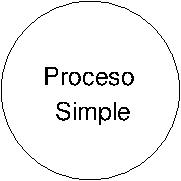
\includegraphics[]{08.Analisis_Funcional/8.2.DFDs/Diagramas/proceso_simple.pdf}
            \caption{Ejemplo de proceso simple.}
            \label{diagramaProcesoSimple}
            \end{center}
         \end{figure}

   \item[Proceso compuesto] El proceso compuesto se representa gráficamente
        mediante un círculo gris y representa lo mismo que el proceso simple con
        la diferencia de que este proceso sí se refinará o descompondrá más en
        el siguiente nivel de abstracción. La figura
        \ref{diagramaProcesoCompuesto} muestra un ejemplo de proceso compuesto.

        \begin{figure}[!ht]
            \begin{center}
            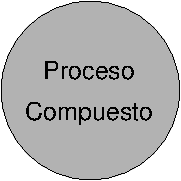
\includegraphics[]{08.Analisis_Funcional/8.2.DFDs/Diagramas/proceso_compuesto.pdf}
            \caption{Ejemplo de proceso compuesto.}
            \label{diagramaProcesoCompuesto}
            \end{center}
         \end{figure}

   \item[Flujo] El flujo se representa gráficamente mediante una flecha que
        entra o sale de un proceso, un almacén o una entidad externa. El flujo
        se utiliza para describir el movimiento de bloques o paquetes de
        información de una parte del sistema a otra. La figura
        \ref{diagramaFlujo} muestra un ejemplo de flujo.

        \begin{figure}[!ht]
            \begin{center}
            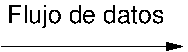
\includegraphics[]{08.Analisis_Funcional/8.2.DFDs/Diagramas/flujo.pdf}
            \caption{Ejemplo de flujo.}
            \label{diagramaFlujo}
            \end{center}
         \end{figure}

   \item[Almacén] El almacén se representa gráficamente mediante dos líneas
        paralelas y se utiliza para modelar una colección de paquetes
        de datos en reposo. La figura \ref{diagramaAlmacen} muestra un ejemplo
        de almacén.

        \begin{figure}[!ht]
            \begin{center}
            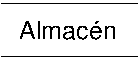
\includegraphics[]{08.Analisis_Funcional/8.2.DFDs/Diagramas/almacen.pdf}
            \caption{Ejemplo de almacén.}
            \label{diagramaAlmacen}
            \end{center}
         \end{figure}

   \item[Entidad externa] La entidad externa es representada gráficamente
        por un rectángulo. Es la fuente o el destino de la información que
        fluye por el sistema. Dicho de otra forma, es un productor o consumidor
        de información que reside fuera de los límites del sistema. La figura
        \ref{diagramaEntidadExterna} muestra un ejemplo de entidad externa.

        \begin{figure}[!ht]
            \begin{center}
            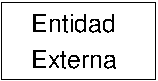
\includegraphics[]{08.Analisis_Funcional/8.2.DFDs/Diagramas/entidad_externa.pdf}
            \caption{Ejemplo de entidad externa.}
            \label{diagramaEntidadExterna}
            \end{center}
         \end{figure}
  \end{description}

\subsection{Nivel de abstracción 0: Diagrama de contexto}

  \paragraph{}En este diagrama se representará el funcionamiento de la
  aplicación de manera general, así como la interacción que mantiene el usuario
  con el sistema por medio de las entidades externas que generan flujos de
  entrada de información (Teclado, Ratón, Sistema y Unidad de almacenamiento) y
  los que reciben y procesan los flujos de salida de información del sistema
  (Pantalla, Impresora). A continuación se describirán las entidades externas
  que intervienen en el Diagrama de contexto.

  \begin{description}
   \item[Teclado] Permitirá al usuario introducir información en el sistema.

   \item[Ratón] Su función será la de permitir al usuario moverse por la
                aplicación.
   \item[Sistema] La información que proporcionará a la aplicación será la fecha
                  y hora del sistema en el que se encuentre instalada.
   \item[Unidad de almacenamiento] Representa toda unidad de almacenamiento
                                   externa que proporcionará archivos tales como
                                   imágenes, archivos pdf, sonidos, etc.
   \item[Servidor] Esta entidad interactúa con la aplicación proporcionando
                   flujos de información de entrada, cuando se le solicita
                   alguna página que tenga almacenada, y flujos de salida,
                   cuando la aplicación realice alguna operación que necesite
                   almacenar una página en el servidor.
   \item[Pantalla] Recibirá los flujos de información de salida de la aplicación
                   y será la encargada de mostrarlos al usuario.
   \item[Impresora] Recibirá información de salida de la aplicación y se
                    encargará de imprimirla en papel.
  \end{description}

  \paragraph{}La figura \ref{diagramaContexto} muestra el Diagrama de contexto.

        \begin{figure}[!ht]
            \begin{center}
            
\includegraphics[]{08.Analisis_Funcional/8.2.DFDs/Niveles/Diagramas/diagrama_contexto.pdf}
            \caption{Diagrama de contexto.}
            \label{diagramaContexto}
            \end{center}
         \end{figure}
\subsection{Nivel de abstracción 1: Módulos principales}

  \paragraph{}El nivel de abstracción 1 muestra una visión general de los
  módulos principales de los que se compone la aplicación: Administrador
  principal, Administrador de centro, Asesores y Alumnos.

  \begin{description}
   \item[Módulo de Administrador principal] Este módulo se encargará de
   crear y mantener toda la estructura básica de la aplicación, gestionando
   al resto de usuarios del sistema, así como los distintos centros,
   titulaciones y asignaturas que se establezcan durante los distintos cursos
   académicos.

   \paragraph{}Recibirá flujos de entrada de información por parte de las
   entidades externas Teclado, Ratón y Sistema. A su vez, también recibirá
   flujos de entrada del almacén Unidad de almacenamiento.

   \paragraph{}Producirá flujos de salida de información tales como mensajes de
   información consultada, mensajes de error, resultados de las operaciones e
   información impresa.

   \paragraph{}La interacción con la base de datos BBDD Asesoría Académica se
   realizará mediante un flujo bidireccional, realizando consultas a la base de
   datos para extraer datos (flujo de entrada) y realizando consultas de
   inserción, modificación y actualización en la base de datos (flujo de
   salida).

   \item[Módulo de Administrador de centro] Este módulo se encargará de
   crear y mantener toda la información relativa a los distintos centros
   que compongan el sistema, gestionando a los usuarios teniendo en cuenta el
   centro al que pertenecen, así como las distintas titulaciones y asignaturas
   que dispongan dichos centros, establecidos durante los distintos cursos
   académicos.

   \paragraph{}Recibirá flujos de entrada de información por parte de las
   entidades externas Teclado y Ratón. A su vez, también recibirá flujos de
   entrada del almacén Unidad de almacenamiento.

   \paragraph{}Producirá flujos de salida de información tales como mensajes de
   información consultada, mensajes de error, resultados de las operaciones e
   información impresa.

   \paragraph{}La interacción con la base de datos BBDD Asesoría Académica se
   realizará mediante un flujo bidireccional, realizando consultas a la base de
   datos para extraer datos (flujo de entrada) y realizando consultas de
   inserción, modificación y actualización en la base de datos (flujo de
   salida).

   \item[Módulo de Asesores] Este módulo se encargará de gestionar a los alumnos
   a los que se preste asesoría, además de crear y mantener las distintas
   plantillas de entrevistas de asesor personales. También será el encargado
   de convocar reuniones en las que participarán los asesores y los alumnos
   que correspondan.

   \paragraph{}Recibirá flujos de entrada de información por parte de las
   entidades externas Teclado y Ratón. A su vez, también recibirá flujos de
   entrada del almacén Unidad de almacenamiento.

   \paragraph{}Producirá flujos de salida de información tales como mensajes de
   información consultada, mensajes de error, resultados de las operaciones e
   información impresa.

   \paragraph{}La interacción con la base de datos BBDD Asesoría Académica se
   realizará mediante un flujo bidireccional, realizando consultas a la base de
   datos para extraer datos (flujo de entrada) y realizando consultas de
   inserción, modificación y actualización en la base de datos (flujo de
   salida).

   \item[Módulo de Alumnos] Este módulo se encargará de gestionar la información
   personal de los alumnos que participarán en la asesoría académica.

   \paragraph{}Recibirá flujos de entrada de información por parte de las
   entidades externas Teclado y Ratón. A su vez, también recibirá flujos de
   entrada del almacén Unidad de almacenamiento.

   \paragraph{}Producirá flujos de salida de información tales como mensajes de
   información consultada, mensajes de error, resultados de las operaciones e
   información impresa.

   \paragraph{}La interacción con la base de datos BBDD Asesoría Académica se
   realizará mediante un flujo bidireccional, realizando consultas a la base de
   datos para extraer datos (flujo de entrada) y realizando consultas de
   inserción, modificación y actualización en la base de datos (flujo de
   salida).
  \end{description}

  \paragraph{}La figura \ref{diagramaNivel1} muestra el nivel de abstracción 1.

        \begin{figure}[!ht]
            \begin{center}
            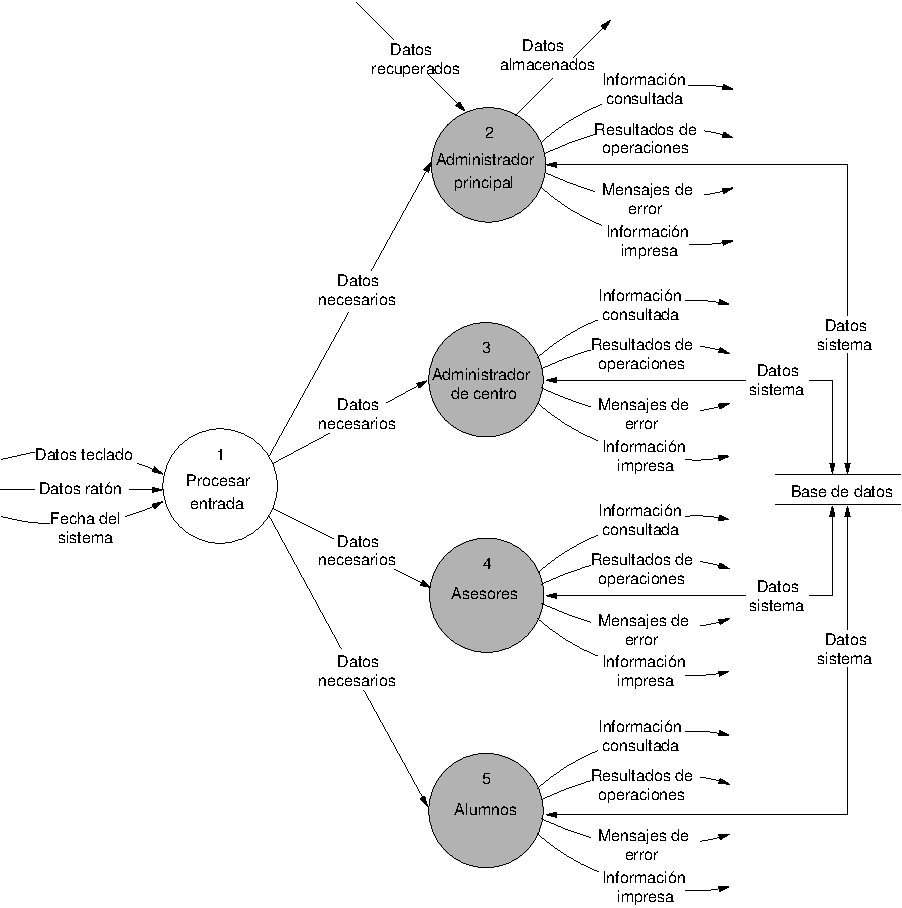
\includegraphics[]{08.Analisis_Funcional/8.2.DFDs/Niveles/Diagramas/nivel1.pdf}
            \caption{Nivel de abstracción 1: Módulos principales.}
            \label{diagramaNivel1}
            \end{center}
         \end{figure}